\section{Introduction}
Learning a good representation in a joint space for vision and language has been a long pursuit in the research of Artificial Intelligence (AI). Recently, the milestone work of CLIP \cite{radford2021learning} from OpenAI demonstrated impressive zero-shot performances across a number of tasks such as image classification on ImageNet~\cite{deng2009imagenet}, Image-to-Text and Text-to-Image retrieval on Flicker-30k ~\cite{young2014image} and MSCOCO\cite{lin2014microsoft, chen2015microsoft}. There has been the pursuit of building contrastive language-image models in other languages such as Italian ~\cite{bianchi2021contrastive}, Korean ~\cite{ko2022large}, Chinese ~\cite{changpinyo2021conceptual, fei2021wenlan, fengshenbang, gu2022wukong, xie2022zero, yang2022chinese} or in a cross-lingual and multilingual setting ~\cite{aggarwal2020towards, carlsson2022cross}.

Training a good language-image representation model often requires a huge amount of text-image pairs and vast computational resources. For instance, CLIP used 400M text-image pairs, and Taiyi ~\cite{fengshenbang}, a recently proposed Chinese model, used 123M text-image pairs. To alleviate this problem, there are multiple works that try to utilize existing pretrained models and only pretrain part of the network ~\cite{portaz2019image, aggarwal2020towards, gu2022wukong, zhai2022lit}. More recently, \newcite{carlsson2022cross} proposed to use Teacher Learning (a.k.a. Knowledge Distillation) on the text encoder of the CLIP model to learn a multilingual text-image representation model. This method only uses machine-translated data from English to a target language, without text-to-image pairs. %We follow this line of work and further improved their method in the following ways.

However, existing works in the cross-lingual or multilingual setting mainly focus on the model's retrieval performance and ignores their generalization ability. The data set to evaluate retrieval performance is often small, e.g., $1,000$ images in test sets for Flickr-30k. The retrieval performance fluctuates acutely with the change in training data distribution. Although current methods achieve good performance in retrieval, these methods often do not perform well on the ImageNet classification tasks. The ability to accurately predict images over $1,000$ classes often indicates better generalization ability of the model. 

\begin{figure*}[t]
\centering
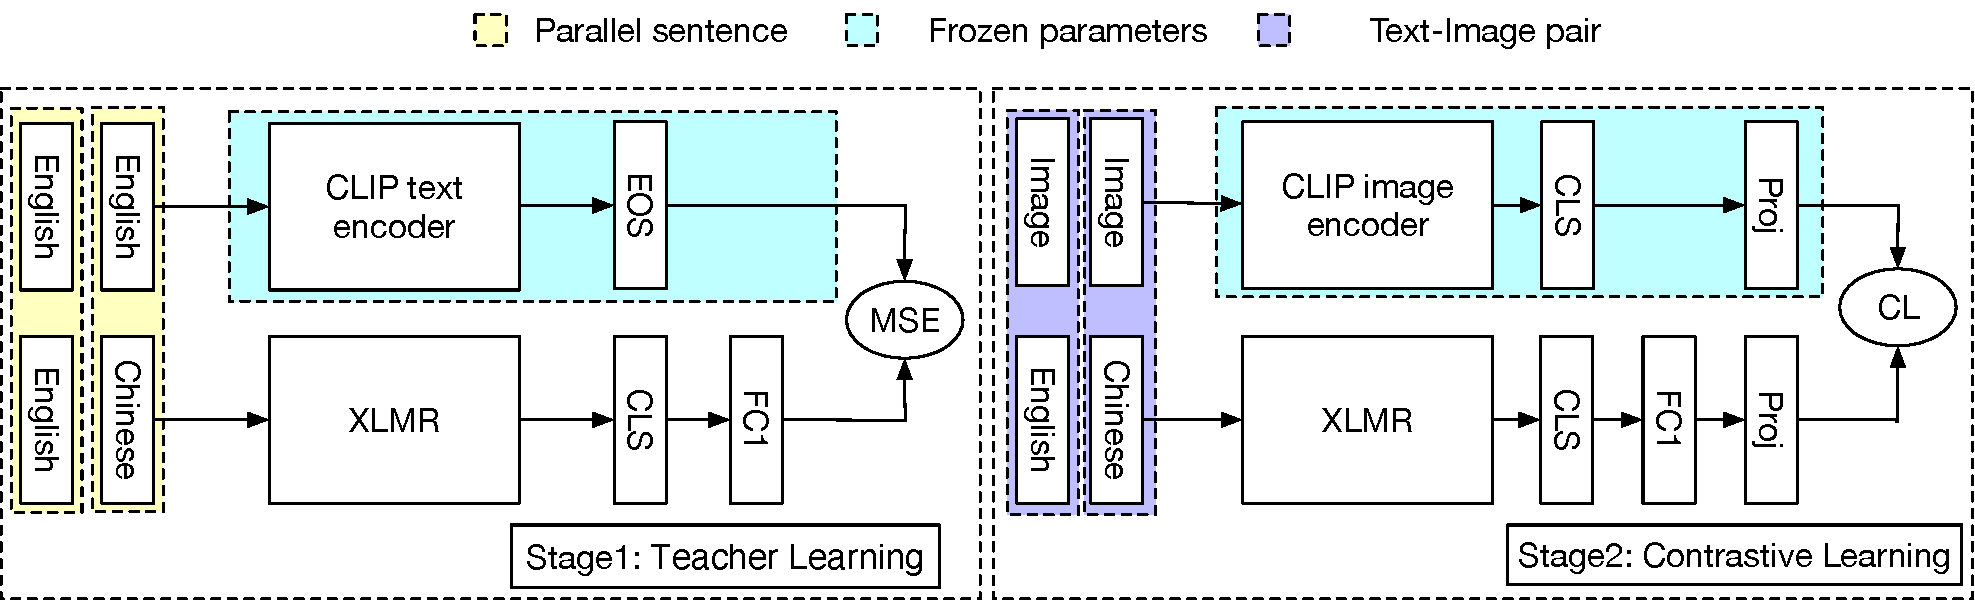
\includegraphics[width=1\textwidth]{distillation-framework.pdf}
\caption{\label{fig:framework}The framework of our method.}
\end{figure*}

To address the aforementioned problems, we propose a bilingual model named Alter ego CLIP (\textbf{AltCLIP}) which achieved strong performances on  ImageNet and multimodal retrieval tasks in both English and Chinese. Our AltCLIP learns a strong bilingual language-image representation under a two-stage framework (see Figure \ref{fig:framework} for an overview). In the first stage, we use Teacher Learning to distill the knowledge learned from CLIP. In the second stage, we train the model via Contrastive Learning ~\cite{hadsell2006dimensionality} on a relatively small amount of Chinese and English text-image pairs. We show the effectiveness of our method by experimenting with a wide range of benchmarks in English and Chinese. Further, We set new state-of-the-art results on multiple image classification and retrieval tasks in Chinese. We further extended this method to train a multilingual multimodal model where we call it AltCLIP$_{M9}$. The AltCLIP$_{M9}$ model achieves state-of-the-art zero-shot results on the multilingual text-image retrieval dataset XTD \cite{aggarwal2020zeroshot}.

%Our contributions includes the following:
%\begin{itemize}
%    \item We propose a simple yet effective two-stage method to train a strong bilingual language-image representation model via teacher learning and contrastive learning;
%    \item We achieved state-of-the-art performance on a set of benchmarks in evaluating Chinese Vision-Language models, out-performing models
%    \item We release a benchmark on Chinese Vision-Language tasks and hope to facilitate the evaluation of Chinese Vision-Language models.
%\end{itemize}

